\documentclass{article}
\usepackage{amsmath}
\usepackage{listings}
\usepackage{graphicx}
\usepackage{float}
\usepackage{booktabs}
\usepackage{geometry}
\usepackage{polski}
\usepackage[hidelinks]{hyperref}
\usepackage[section]{placeins}
\usepackage[T1]{fontenc}
% Ustawienia marginesów
\geometry{top=3cm,bottom=2cm,left=2cm,right=2cm}

\title{Dokumentacja Projektu Zaliczeniowego\\ \huge Baza danych dla firmy Wombat Grylls sp. z o.o.}
\author{Kacper Daniel, Tadeusz Jagniewski, Paweł Karwecki, Piotr Marciniak, Konrad Mądry}
\date{\today}

\begin{document}

\maketitle

\newpage

\tableofcontents
\newpage

\section{Spis użytych technologii}
\begin{itemize}
    \item System zarządzania bazą danych: MariaDB
    \item Język programowania: Python (do generowania danych, spis bibliotek znajduje się w 
pliku \texttt{requirements.txt})
    \item Narzędzie do analizy, generowania wykresów i raportowania: R Markdown (wszystkie
biblioteki znajdują się w pliku \texttt{raport\_team03})
    \item Format raportu: PDF
\end{itemize}

\section{Lista plików i opis ich zawartości}
\begin{itemize}
    \item \texttt{category\_fill.py} - Skrypt łączący się z bazą danych MySQL i wstawiający listę kategorii podróży,
    \item \texttt{generowanie\_tabel.py} - Skrypt generujący dane i tabele potrzebne do bazy danych,
    \item \texttt{database\_filler\_template.py} - Skrypt wstawiający wygenerowane dane do bazy danych,
    \item \texttt{tabele.sql} - Plik sql tworzący potrzebne tabele,
    \item \texttt{tabele.py} - Skrypt wykonujący zapytania z \texttt{tabele.sql} na bazie danych,
    \item \texttt{wszystko.py} - Skrypt uruchamiający skrypty \texttt{tabele.py}, \texttt{category\_fill.py} i \texttt{database\_filler\_template.py},
    \item \texttt{requirements.txt} - Lista bibliotek Pythona i ich wersji, wymaganych do uruchomienia projektu,
    \item \texttt{raport\_team03.Rmd} - Plik generujący raport,
    \item \texttt{raport\_team03.pdf} - Raport w formacie PDF,
    \item \texttt{Adresy\_StanNa20250119.csv} - Zbiór wszystkich adresów we Wrocławiu,
    \item \texttt{lista\_imion.csv} - Zbiór polskich imion z częstością występowania,
    \item \texttt{lista\_nazwisk.csv} - Zbiór polskich nazwisk z częstością występowania,
    \item \texttt{dokumentacja.pdf} - Dokumentacja projektu.
\end{itemize}

\section{Kolejność i sposób uruchamiania plików}
\begin{enumerate}
    \item Otwieramy cały folder z plikami w VS Code \\
	\item Pobieramy biblioteki komendą \texttt{pip install -r requirements.txt} poprzez terminal w VS Code \\
	\item Uruchamiamy plik \texttt{wszystko.py}, aby utworzyć i wpisać nowe dane do tabeli \\
	\item Otwieramy plik \texttt{raport\_team03.Rmd} w RStudio i klikamy w opcję 'Knit' \\
	\item Włączamy gotowy raport \texttt{raport\_team03.pdf}
\end{enumerate}

\section{Schemat projektu bazy danych}
\begin{figure}[h!]
\centering
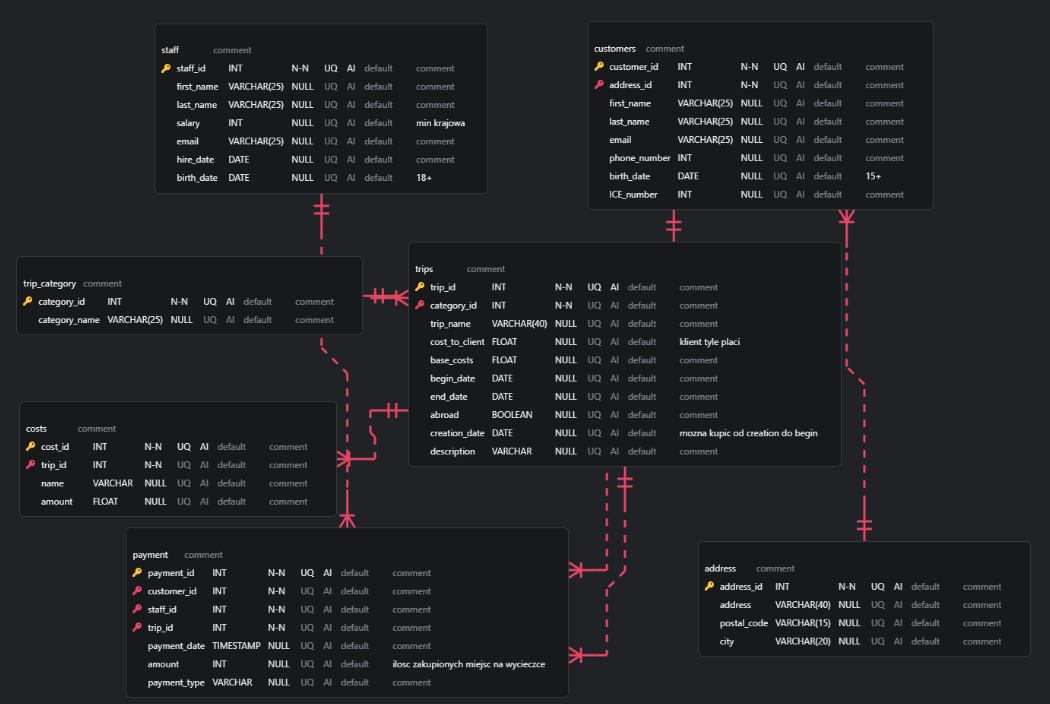
\includegraphics[width=\textwidth]{schemat_bazy.png}  % Podmień na odpowiednią ścieżkę do pliku z schematem
\caption{Schemat bazy danych firmy Wombat Grylls sp. z o.o.}
\end{figure}

\newpage

\section{Lista zależności funkcyjnych dla każdej relacji}

\subsection{Tabela: Address}
\begin{itemize}
    \item address\_id $\rightarrow$ address, postal\_code, city
\end{itemize}
\subsection{Tabela: Costs}
\begin{itemize}
    \item cost\_id $\rightarrow$ trip\_id, name, amount
    \item trip\_id $\rightarrow$ trip\_id (odwołanie do tabeli trips)
\end{itemize}
\subsection{Tabela: Customers}
\begin{itemize}
    \item customer\_id $\rightarrow$ address\_id, first\_name, last\_name, email, phone\_number, amount, birth\_date, ICE\_number
    \item address\_id $\rightarrow$ address\_id (odwołanie do tabeli address)
\end{itemize}
\subsection{Tabela: Payment}
\begin{itemize}
    \item payment\_id $\rightarrow$ customer\_id, staff\_id, trip\_id, payment\_date, amount
    \item customer\_id $\rightarrow$ customer\_id (odwołanie do tabeli customers)
    \item staff\_id $\rightarrow$ staff\_id (odwołanie do tabeli staff)
    \item trip\_id $\rightarrow$ trip\_id (odwołanie do tabeli trips)
\end{itemize}
\subsection{Tabela: Staff}
\begin{itemize}
    \item staff\_id $\rightarrow$ address\_id, first\_name, last\_name, salary, email, hire\_date, birth\_date
    \item address\_id $\rightarrow$ address\_id (odwołanie do tabeli address)
\end{itemize}
\subsection{Tabela: Trips}
\begin{itemize}
    \item trip\_id $\rightarrow$ category\_id, trip\_name, cost\_to\_client, begin\_date, end\_date, abroad, creation\_date, description
    \item category\_id $\rightarrow$ category\_id (odwołanie do tabeli trip\_category)
\end{itemize}
\subsection{Tabela: Trip\_category}
\begin{itemize}
    \item category\_id $\rightarrow$ category\_name
\end{itemize}

\newpage

\section{Uzasadnienie, że baza jest w EKNF}
Baza danych została zaprojektowana zgodnie z zasadami EKNF (Efektywnej Normalnej Formy Encji). W każdej tabeli spełnione są następujące warunki:
\begin{itemize}
    \item Każda tabela posiada jednoznaczny klucz główny.
    \item Brak zależności przechodnich - wszystkie zależności funkcyjne są określone przez klucze obce.
    \item Zależności funkcyjne są zgodne z zasadami normalizacji, eliminując redundancję.
\end{itemize}

\section{Opis trudności podczas realizacji projektu}
Najtrudniejszym elementem było generowanie danych. Musieliśmy przyjąć pewne uproszczenia, które spowodowały, że baza nie jest tak realistyczna, jak mogłaby być w prawdziwym życiu. 

\end{document}
